
\chapter{Космические корабли и станции. Современные реалии 50-летней давности.}
\label{ch:spacecraft-space-station}

Глава посвящена исследованию космических кораблей и станций на основе базы знаний международного проекта Викиданные. С помощью SPARQL-скриптов построен список отечественных кораблей и станций, а также временные графики запуска кораблей в нашей стране и в мире, за период с 1960 по 2021 год. Выполнена оценка полноты Викиданных, показавшая, что многие объекты имеют неправильное значение свойства <<частный случай понятия (P31)>>.
\marginnote{\wdProperty{31}{Частный случай понятия} это то же, что и экземпляр \wdProperty{31}{instance of}}
\section{Экземпляры объекта <<Космические корабли>> и <<Космические станции>>}
Исследуется свойство \wdProperty{31}{частный случай понятия} и объекты \href{https://www.wikidata.org/wiki/Q25956}{космические станции (Q25956)} и \href{https://www.wikidata.org/wiki/Q40218}{космические корабли (Q40218)}.
Построим список всех космических кораблей с помощью листинга~\ref{lst:spaceships}.

\marginnote{\index{Космические корабли и станции!Определения!Космический корабль}Космический корабль ~--- устройство, используемое для выполнения задач в космическом пространстве.}

\begin{lstlisting}[ language=SPARQL, numbers=none, caption={{\href{https://w.wiki/4By4}{Список кораблей}}\protect\footnotemark}, label=lst:spaceships, ]
# List of spacecraft (Q40218) and space station (Q25956)
SELECT  ?s ?sLabel ?typeLabel
WHERE
{
  VALUES ?type {wd:Q40218 wd:Q25956}
  ?s wdt:P31 ?type.  # Selecting the type of object
  SERVICE wikibase:label {bd:serviceParam wikibase:language"ru,en"}
}
\end{lstlisting}
\footnotetext{Найдено \num{118} объектов в 2021 году. Ссылка на SPARQL-запрос: \href{https://w.wiki/4By4}{https://w.wiki/4By4}}
\section{Хорошие и плохие объекты}
По состоянию на 2021 год на Викиданных наиболее полным и проработанным является космический корабль \href{ https://www.wikidata.org/wiki/Q184201}{Apollo 8}, имеющий 30 свойств\autocite{spacecraftProWD} .
При этом всего одно свойство имеет ряд кораблей: \href{https://www.wikidata.org/wiki/Q10491365}{ Europa Astrobiology Lander}, \href{https://www.wikidata.org/wiki/Q6514453 }{ Project Orbiter}, \href{https://www.wikidata.org/wiki/Q5961734 }{ LRK}, \href{https://www.wikidata.org/wiki/Q5327028 }{ EarthForce One}, \href{https://www.wikidata.org/wiki/Q60767924 }{ Союз ГВК}, \href{https://www.wikidata.org/wiki/Q22907583 }{ CubeSat for Solar Particles}\autocite{spacecraftProWD} .
Для изучения объектов использовался сервис ProWD и соответствующий запрос \autocite{spacecraftProWD} . Заполнение объктов неравномерное, большая часть заполнены менее, чем на 30\%\autocite{spacecraftProWD} . 

\section{Список отечественных кораблей}
Найдём корабли, сконструированные в СССР или России с помощью скрипта~\ref{lst:spaceshipsUSSR}:

\begin{lstlisting}[ language=SPARQL, numbers=none, caption={{\href{https://w.wiki/4BbY}{Список отечественных кораблей}}\protect\footnotemark}, label=lst:spaceshipsUSSR, ]
# List of Russian and USSR spacecraft
SELECT  ?spacecraft  ?spacecraftLabel 
WHERE
{
  {?spacecraft wdt:P31 wd:Q40218.} UNION #spacecraft
  {?spacecraft wdt:P31 wd:Q18039177.} UNION #fictional spacecraft
  {?spacecraft wdt:P31 wd:Q402330.}#robotic spacecraft
  {?spacecraft wdt:P17 wd:Q15180. } UNION #USSR
  {?spacecraft wdt:P17 wd:Q159. } #Russia
  SERVICE wikibase:label {bd:serviceParam wikibase:language"ru,en"}
}
\end{lstlisting}
\footnotetext{Найдено три отечественных корабля в 2017 году и \num{21}  в 2021 году. Ссылка на SPARQL-запрос: \href{https://w.wiki/4BbY}{https://w.wiki/4BbY}}

\section{Анализ полноты Викиданных}
До полноты Викиданным в области космических кораблей и станций крайне далеко. Если по запросу обо всех кораблях вывелось 193 результата, то по запросу об отечественных кораблях всего 21. Это говорит о том, что данные не полны. В статьях русской Википедии \href{https://ru.wikipedia.org/wiki/%D0%9A%D0%BE%D1%81%D0%BC%D0%B8%D1%87%D0%B5%D1%81%D0%BA%D0%B0%D1%8F_%D0%BF%D1%80%D0%BE%D0%B3%D1%80%D0%B0%D0%BC%D0%BC%D0%B0_%D0%A1%D0%A1%D0%A1%D0%A0}{Космическая программа СССР} и \href{https://ru.wikipedia.org/wiki/%D0%9A%D0%BE%D1%81%D0%BC%D0%BE%D0%BD%D0%B0%D0%B2%D1%82%D0%B8%D0%BA%D0%B0_%D0%A0%D0%BE%D1%81%D1%81%D0%B8%D0%B8}{Космонавтика России} можно насчитать как минимум 45 космических кораблей, спроектированных в СССР и России. То есть в Викиданных представлено менее половины от всех отечественных кораблей, однако ситуация в 2021 стала значительно лучше по сравнению с 2017 годом, когда по запросу ~\ref{lst:spaceshipsUSSR} выдавалось менее 10\% от всех кораблей. 

\section{Временные графики освоения космоса в нашей стране и мире}

%%%%%%%%%%%%%%%% Упражнение 1 %%%%%%%%%%%%%%%% 
\marginnote{
Сколько кораблей было запущено в СССР в следующие десятилетия?
\begin{itemize}
\item 1960-е
\item 1970-е
\item 1980-е
\end{itemize}
См. ответ~\ref{answer:launches_USSR} на с.~\pageref{answer:launches_USSR}.
}

Скрипт построения графика запуска космических аппаратов в нашей стране, начиная с 1960-х годов, представлен в листинге~\ref{lst:imageRU}.
\begin{lstlisting}[ language=SPARQL, caption={{\href{https://w.wiki/4QGX}{Запуски космический кораблей в СССР и России}}\protect\footnotemark}, label=lst:imageRU, ]
# The number of spacecraft launches in Russia every 5 years
#defaultView:BarChart
SELECT (STR(?lapse) AS ?lapse_str) (COUNT(?item) AS ?quantity)
WHERE {                  # spacecraft belongs to
        {?item wdt:P17 wd:Q15180} # Soviet Union
  UNION {?item wdt:P17 wd:Q159}.  # or Russia
  
  ?item wdt:P619 ?launch. # date of spacecraft launch (P619)
  BIND( YEAR(?launch) AS ?year) 
  BIND(FLOOR(?year/5)*5 AS ?lapse) # count for each 5 years
SERVICE wikibase:label {bd:serviceParam wikibase:language "ru,en"}
} 
GROUP BY ?lapse
ORDER BY ?lapse # Order 1970, 1975, 1980, ...
\end{lstlisting}
\footnotetext{Найдено \num{14} результата в 2021 г. Ссылка на SPARQL-запрос: \href{https://w.wiki/4QGX}{https://w.wiki/4QGX}}
\wdProperty{619}{Свойство} (дата запуска космического корабля) позволяет получать количество запусков кораблей в указанный период, что в рамках данного скрипта заменяет набор \wdProperty{31}{свойств} (частный случай понятия), то есть поиск кораблей по свойству <<запуск>> позволяет отказаться от использования свойства \wdProperty{31}{экземпляр} космического корабля. В случае отсутствия функции {\it STR} в третьей строке, год запуска ({\it lapse}) рассматривается как число, что нежелательным образом приводит столбчатую диаграмму к виду графика, где горизонтальная ось отвечает за год запуска, а результаты обозначаются точками с координатами (год, запуски). Логический оператор {\it UNION} в строках пять и шесть позволяет объединить запуски России и СССР. В строке 10 производится подсчёт количества за пятилетку, от года Х до Х+5. В строке 13 результаты группируются по пятилеткам. Переменная {\it lapse} отвечает за накопление данных за период, переменная quantity указывает, что в рамках скрипта требуется воспринимать объекты как их количество.

%%%%%%%%%%%%%%%% Упражнение 2 %%%%%%%%%%%%%%%% 
\marginnote{
В каких из следующих десятилетий человечестро совершило наибольшее и наименьшее количество запусков космических кораблей?
\begin{itemize}
\item 1970-е
\item 1980-е
\item 1990-е
\item 2000-е
\end{itemize}
См. ответ~\ref{answer:launches_world} на с.~\pageref{answer:launches_world}.
}

\begin{figure*}[h!]
  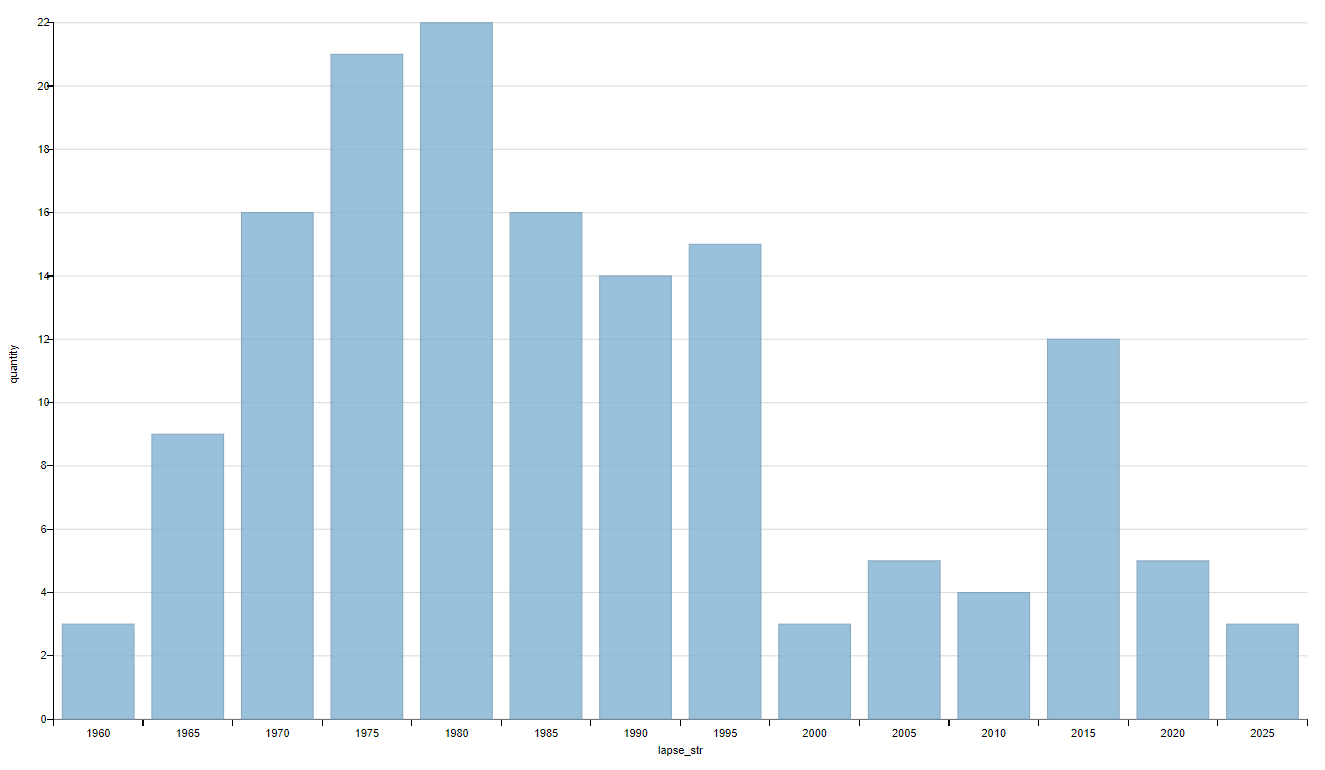
\includegraphics[width=\linewidth]{graphics/chapter/spacecraft_space_station/ImgRU.png}
  \caption[График Россия]{Визуализация количества запусков космических кораблей а России каждые 5 лет 2021 SPARQL}%
  \label{fig:ImageRU5}%
\end{figure*}

Из графика ~\ref{fig:ImageRU5} можно увидеть, что самый активный период развития космонавтики в нашей стране был в 1970-1995 годах.
Скрипт построения графика запусков космический кораблей в мире по годам и странам представлен в листинге ~\ref{lst:imageALL}:
\begin{lstlisting}[ language=SPARQL, numbers=none, caption={{\href{https://w.wiki/4bEu}{Запуски космических кораблей в мире}}\protect\footnotemark}, label=lst:imageALL, ]
# Diagram of spacecraft launches by year and country
#defaultView:BarChart
SELECT ?year (COUNT(?obj) AS ?count) ?country ?countryLabel
WHERE {
  ?obj wdt:P17 ?country. # spacecraft belongs to country 
  ?obj wdt:P619 ?launch. # date of spacecraft launch
  BIND(str(YEAR(?launch)) AS ?year)
  
  SERVICE wikibase:label {bd:serviceParam wikibase:language "ru".}
}
GROUP BY ?year ?country ?countryLabel
\end{lstlisting}
\footnotetext{Найдено \num{328} результата в 2021 г. Ссылка на SPARQL-запрос: \href{https://w.wiki/4bEu}{https://w.wiki/4bEu}}

\begin{figure*}[h!]
  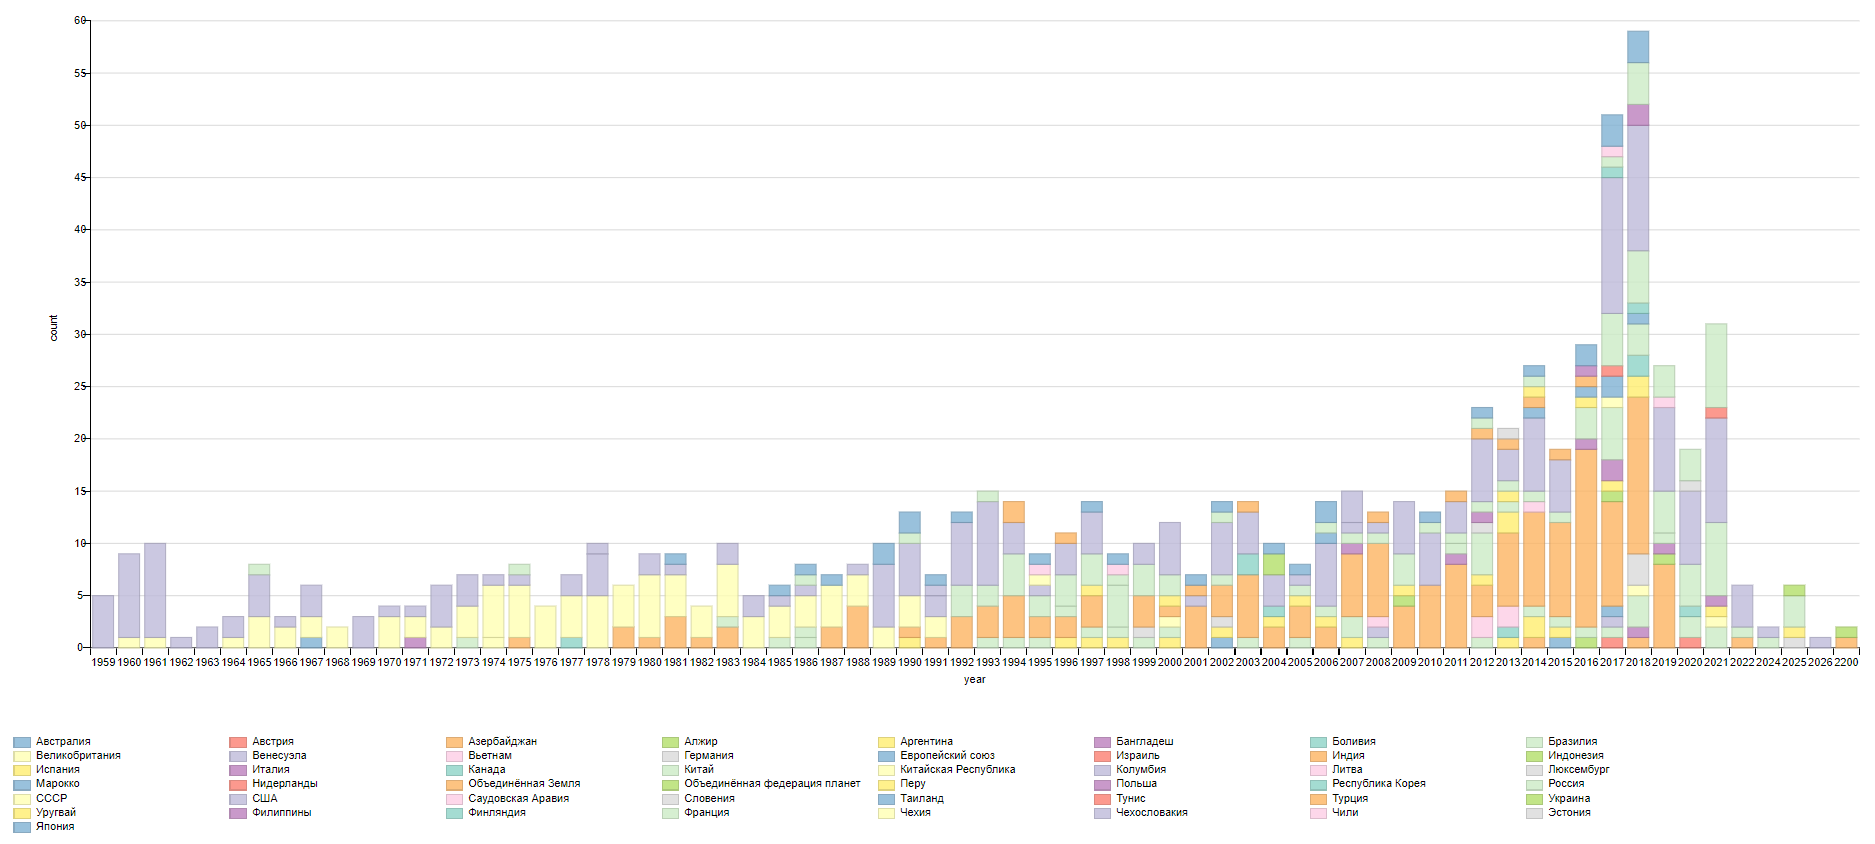
\includegraphics[width=\linewidth]{graphics/chapter/spacecraft_space_station/Visualization of the number of spacecraft launches by year and country 2021.png}
  \caption[График мир]{Визуализация количества запусков космических кораблей по годам и странам 2021 SPARQL}%
  \label{fig:ImgALL}%
\end{figure*}

%%%%%%%%%%%%%%%% Упражнение 3 %%%%%%%%%%%%%%%% 
\marginnote{
Какие из следующих стран являются рекордсменами по количеству запусков в год в период 2015-2020 годов согласно данным в Викиданных?
\begin{itemize}
\item Россия
\item США
\item Индия
\item Китай
\end{itemize}
См. ответ~\ref{answer:launches_country} на с.~\pageref{answer:launches_country}.
}

Из графика ~\ref{fig:ImgALL} можно увидеть, что по состоянию на 2021 год в Викиданных превалируют данные о запусках США и Индии (только у них зафиксировано более 10 графков в год) в 2017-2018 годах. Пик запусков был в 2018 году (59 запусков). По информации из Викиданных российская космонавтика занимает средние позиции по количеству запусков, её численные показатели за последние 5 лет схожи с показателями СССР 1975-1980 годов и составляют около 5 запусков в год.

\section{Упражнения}
\begin{itemize}
  \item Подсчитать и вывести список кораблей, которые отправились или планируется отправить на \wdqName{Марс}{111}.
  \item Подсчитать и построить график доли кораблей, предназначенных для отправки на \wdqName{Марс}{111}, по отношению к кораблям отправленным на \wdqName{Луну}{405}.
  \item Посчитать количество \wdqName{успешных}{7632586} запусков относительно \wdqName{провальных}{1121708}. В викиданных их количество указывается в свойствах космической программы, например, \wdqName{космическая программа <<Луна>>}{192372}. 
\end{itemize}
